\input{header}
\AtBeginSection[]
{
	\begin{frame}<beamer>
		\frametitle{Outline}
		\tableofcontents[current,currentsubsection]
	\end{frame}
}

\begin{document}


\begin{frame}[allowframebreaks] \frametitle{What is a computer}
  \begin{itemize}  
  \item Computers are complicated, but we can
    construct idealized computational models to do analysis

  \item Finite automata are the idealized model that we will discuss
    
\item Example: automatic door


  Fig 1.1

  \begin{center}
    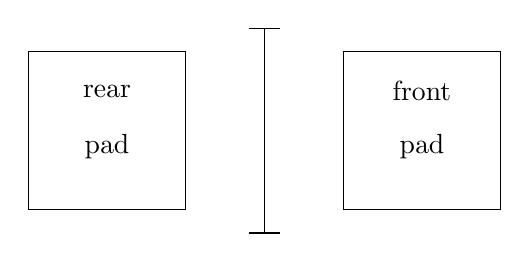
\begin{tikzpicture}
\tikzset{-}
    \draw (-0.2,1.3) -- (0.2,1.3);
\draw (-0.2,-1.3) -- (0.2,-1.3);    
\draw (0,-1.3) -- (0,1.3);
\draw (1,-1) rectangle (3,1);
\path node at (2, 0.5) {front};
\path node at (2, -0.2) {pad};
\draw (-1,-1) rectangle (-3,1);
\path node at (-2, 0.5) {rear};
\path node at (-2, -0.2) {pad};
  \end{tikzpicture}
\end{center}
\item Rules:

\item [] When it moves, it cannot hit people
\item We can use a simple graph to summarize all operations
\item Fig 1.2

\begin{tikzpicture}
\node[state] (closed) {closed};
  \node[state] (open) [right of=closed] {open};

   \path (closed) edge[loop below]  node {rear, both, neither} (closed)
         (closed) edge[bend left, above]              node {front} (open)
         (open) edge[bend left, below]              node {neither} (closed)
         (open) edge[loop right] node {front, rear, both} (open);
\end{tikzpicture}

\item Single bit memory (open and closed)
\item Automaton (single)

\item [] automata (plural)

\end{itemize}\end{frame} \begin{frame}[allowframebreaks] \frametitle{Examples of automata}
  \begin{itemize}
  \item Fig 1.4: a state diagram

  \begin{tikzpicture}
  \node[state,initial] (q_1) {$q_1$};
  \node[state,accepting, right of=q_1] (q_2)  {$q_2$};
  \node[state, right of=q_2] (q_3)  {$q_3$};

  \draw (q_1) edge[loop above]    node {$0$} (q_1)
        (q_1) edge[above]  node {$1$} (q_2)
        (q_2) edge[loop above]    node {$1$} (q_2)
        (q_2) edge[bend left, above] node {$0$} (q_3)
        (q_3) edge[bend left, below] node {$0,1$} (q_2);
\end{tikzpicture}

\item [] states: $q_1, q_2, q_3$

\item [] starting states: $q_1$

\item [] accept state $q_2$ (double circle)
\item Example: running an input string 1101
  \begin{equation*}
    q_1
\rightarrow q_2 \rightarrow
q_2 \rightarrow q_3 
\rightarrow q_2
\end{equation*}
This string is accepted
\item Example: running 10
    \begin{equation*}
    q_1
\rightarrow q_2 \rightarrow
q_3 
\end{equation*}
$q_3$ is not an accept state, so the string is rejected
\item What are all strings accepted?
\item [] We will say what this set is
\item [] Unfortunately, it may not be always easy to know the set

\end{itemize}\end{frame}


\begin{frame}[allowframebreaks] \frametitle{Formal definition}
We formally define a state diagram as a 5-tuple $(Q,\Sigma, \delta, q_0, F)$
  \begin{itemize}

\item $Q$: set of states. It is a \alert{finite} set
\item $\Sigma$: alphabet (i.e., set of characters in input string). It is a finite set
\item $\delta: Q \times \Sigma \rightarrow Q$: transition function
\item [] This is the most complicated part of the definition. We explain it by an example
  later
\item $q_0 \in Q$: start state
\item $F \subset Q$: set of accept states

\item For the example given above,
\begin{gather*}
  Q=\{q_1,q_2, q_3\}\\
\Sigma=\{0,1\}\\
q_0 = q_1 \\
F=\{q_2\}
\end{gather*}
\item The $\delta$ function:
  \begin{center}
  \begin{tabular}{c|cc}
& 0 & 1\\ \hline
$q_1$ & $q_1$ & $q_2$\\
$q_2$ & $q_3$ & $q_2$\\
$q_3$ & $q_2$ & $q_2$
  \end{tabular}
\end{center}
\item Language of $M$: all strings accepted by $M$. 
Denoted as
\begin{equation*}
A=L(M)
\end{equation*}
\item Figure 1.4:
  \begin{equation*}
    \begin{split}
    A=\{
w \mid & w: \text{ at least one 1, even \# 0} \\
& \text{after the last 1}\}
\end{split}
  \end{equation*}
\end{itemize}
\end{frame}

\begin{frame}[allowframebreaks] \frametitle{Example 1.7}
  \begin{itemize}
  \item Figure 1.8

    \begin{tikzpicture}
\node[state,initial] (q_1) {$q_1$};
\node[state,accepting] (q_2) [right of=q_1] {$q_2$};      

  \path (q_1) edge[bend left, above]  node {$1$} (q_2)
        (q_1) edge[loop above] node {$0$} (q_1)
        (q_2) edge[loop above] node {$1$} (q_2)
        (q_2) edge[bend left, below]  node {$0$} (q_1);
      \end{tikzpicture}
\item $M=(\{q_1,q_2\}, \{0,1\},
\delta, q_1, \{q_2\})$
\item What is $L(M)$ ?
Anything ends with 1

\item How to think about this ?

\item Before the last input character, we must
  be at $q_1$ or $q_2$. Then only if the last is 1 we
  can reach $q_2$ to get accepted
\end{itemize}\end{frame}

\end{document}
